\section{Teorie ke zpracování}

Tato práce se zabývá porovnáním vlastností základních konformních zobrazení a vyhodnocení jejich využitelnosti pro mapování konkrétně vymezené oblasti. Zhodnocení vhodnosti zobrazení se opírá primárně o analýzu délkového zkreslení, které je zkoumáno podél okrajových rovnoběžek zadaného území. Analýza se zaměřuje na zobrazení v obecné poloze, konkrétně na válcovou a kuželovou projekci (obě se dvěma nezkreslenými rovnoběžkami) a na zobrazení stereografické.

\textbf{Přehled použitého značení}
V rámci matematických formulací je využívána následující symbolika:
\begin{itemize}
    \item $R$ definuje poloměr referenční koule.
    \item $u, v$ reprezentují zeměpisné souřadnice, zatímco $\check{s}, d$ slouží pro souřadnice kartografické.
    \item $x, y$ určují polohu bodu v pravoúhlé souřadnicové soustavě mapy.
    \item $u_0, u_1, u_2$ a $\check{s}_0, \check{s}_1, \check{s}_2$ označují zeměpisné, respektive kartografické šířky rovnoběžek s nulovým zkreslením.
    \item $K = [u_k, v_k]$ určuje pozici kartografického pólu a $u_s$ šířku severní hranice území.
\end{itemize}

\subsection{Válcové konformní zobrazení}
Mercatorovo zobrazení v obecné poloze je matematicky popsáno následujícími rovnicemi:
$$x = c \cos d$$ 
$$y = R \ln \tan\left(\frac{\check{s}}{2} + 45^\circ\right)$$ 
kde parametr $c = R \cos \check{s}_0$ a hodnota $\check{s}_0$ představuje šířku rovnoběžky, na které nedochází ke zkreslení. 

Aby bylo zobrazení optimální, požadujeme symetrické rozložení extrémů zkreslení. Délkové zkreslení na severním ($m_r^s$) a jižním ($m_r^j$) okraji oblasti tak musí být co do velikosti odchylky shodné se zkreslením na rovníku ($m_r^r$), avšak s opačným znaménkem. To vyjadřují vztahy:
$$m_r^s = m_r^j = 1 + \nu, \quad m_r^r = 1 - \nu$$ 
Z čehož vyplývá součet $m_r^s + m_r^r = 2$.

Měřítko délek na konkrétní kartografické rovnoběžce lze vyjádřit vzorcem:
$$m_r = \frac{\cos \check{s}_0}{\cos \check{s}}$$ 
Pomocí okrajové šířky $\check{s}_s$ pak můžeme definovat nezkreslenou rovnoběžku vztahem:
$$\cos \check{s}_0 = \frac{2 \cos \check{s}_s}{1 + \cos \check{s}_s}$$ 
Zkoumanou oblast je nutné ohraničit dvěma kartografickými rovnoběžkami tak, aby tvořily co nejužší pás ohraničující dané území. Hodnotu samotného zkreslení $\nu$ získáme odečtením jedničky od měřítka délek ($\nu = m - 1$).

 \begin{figure}[h!]
\centering
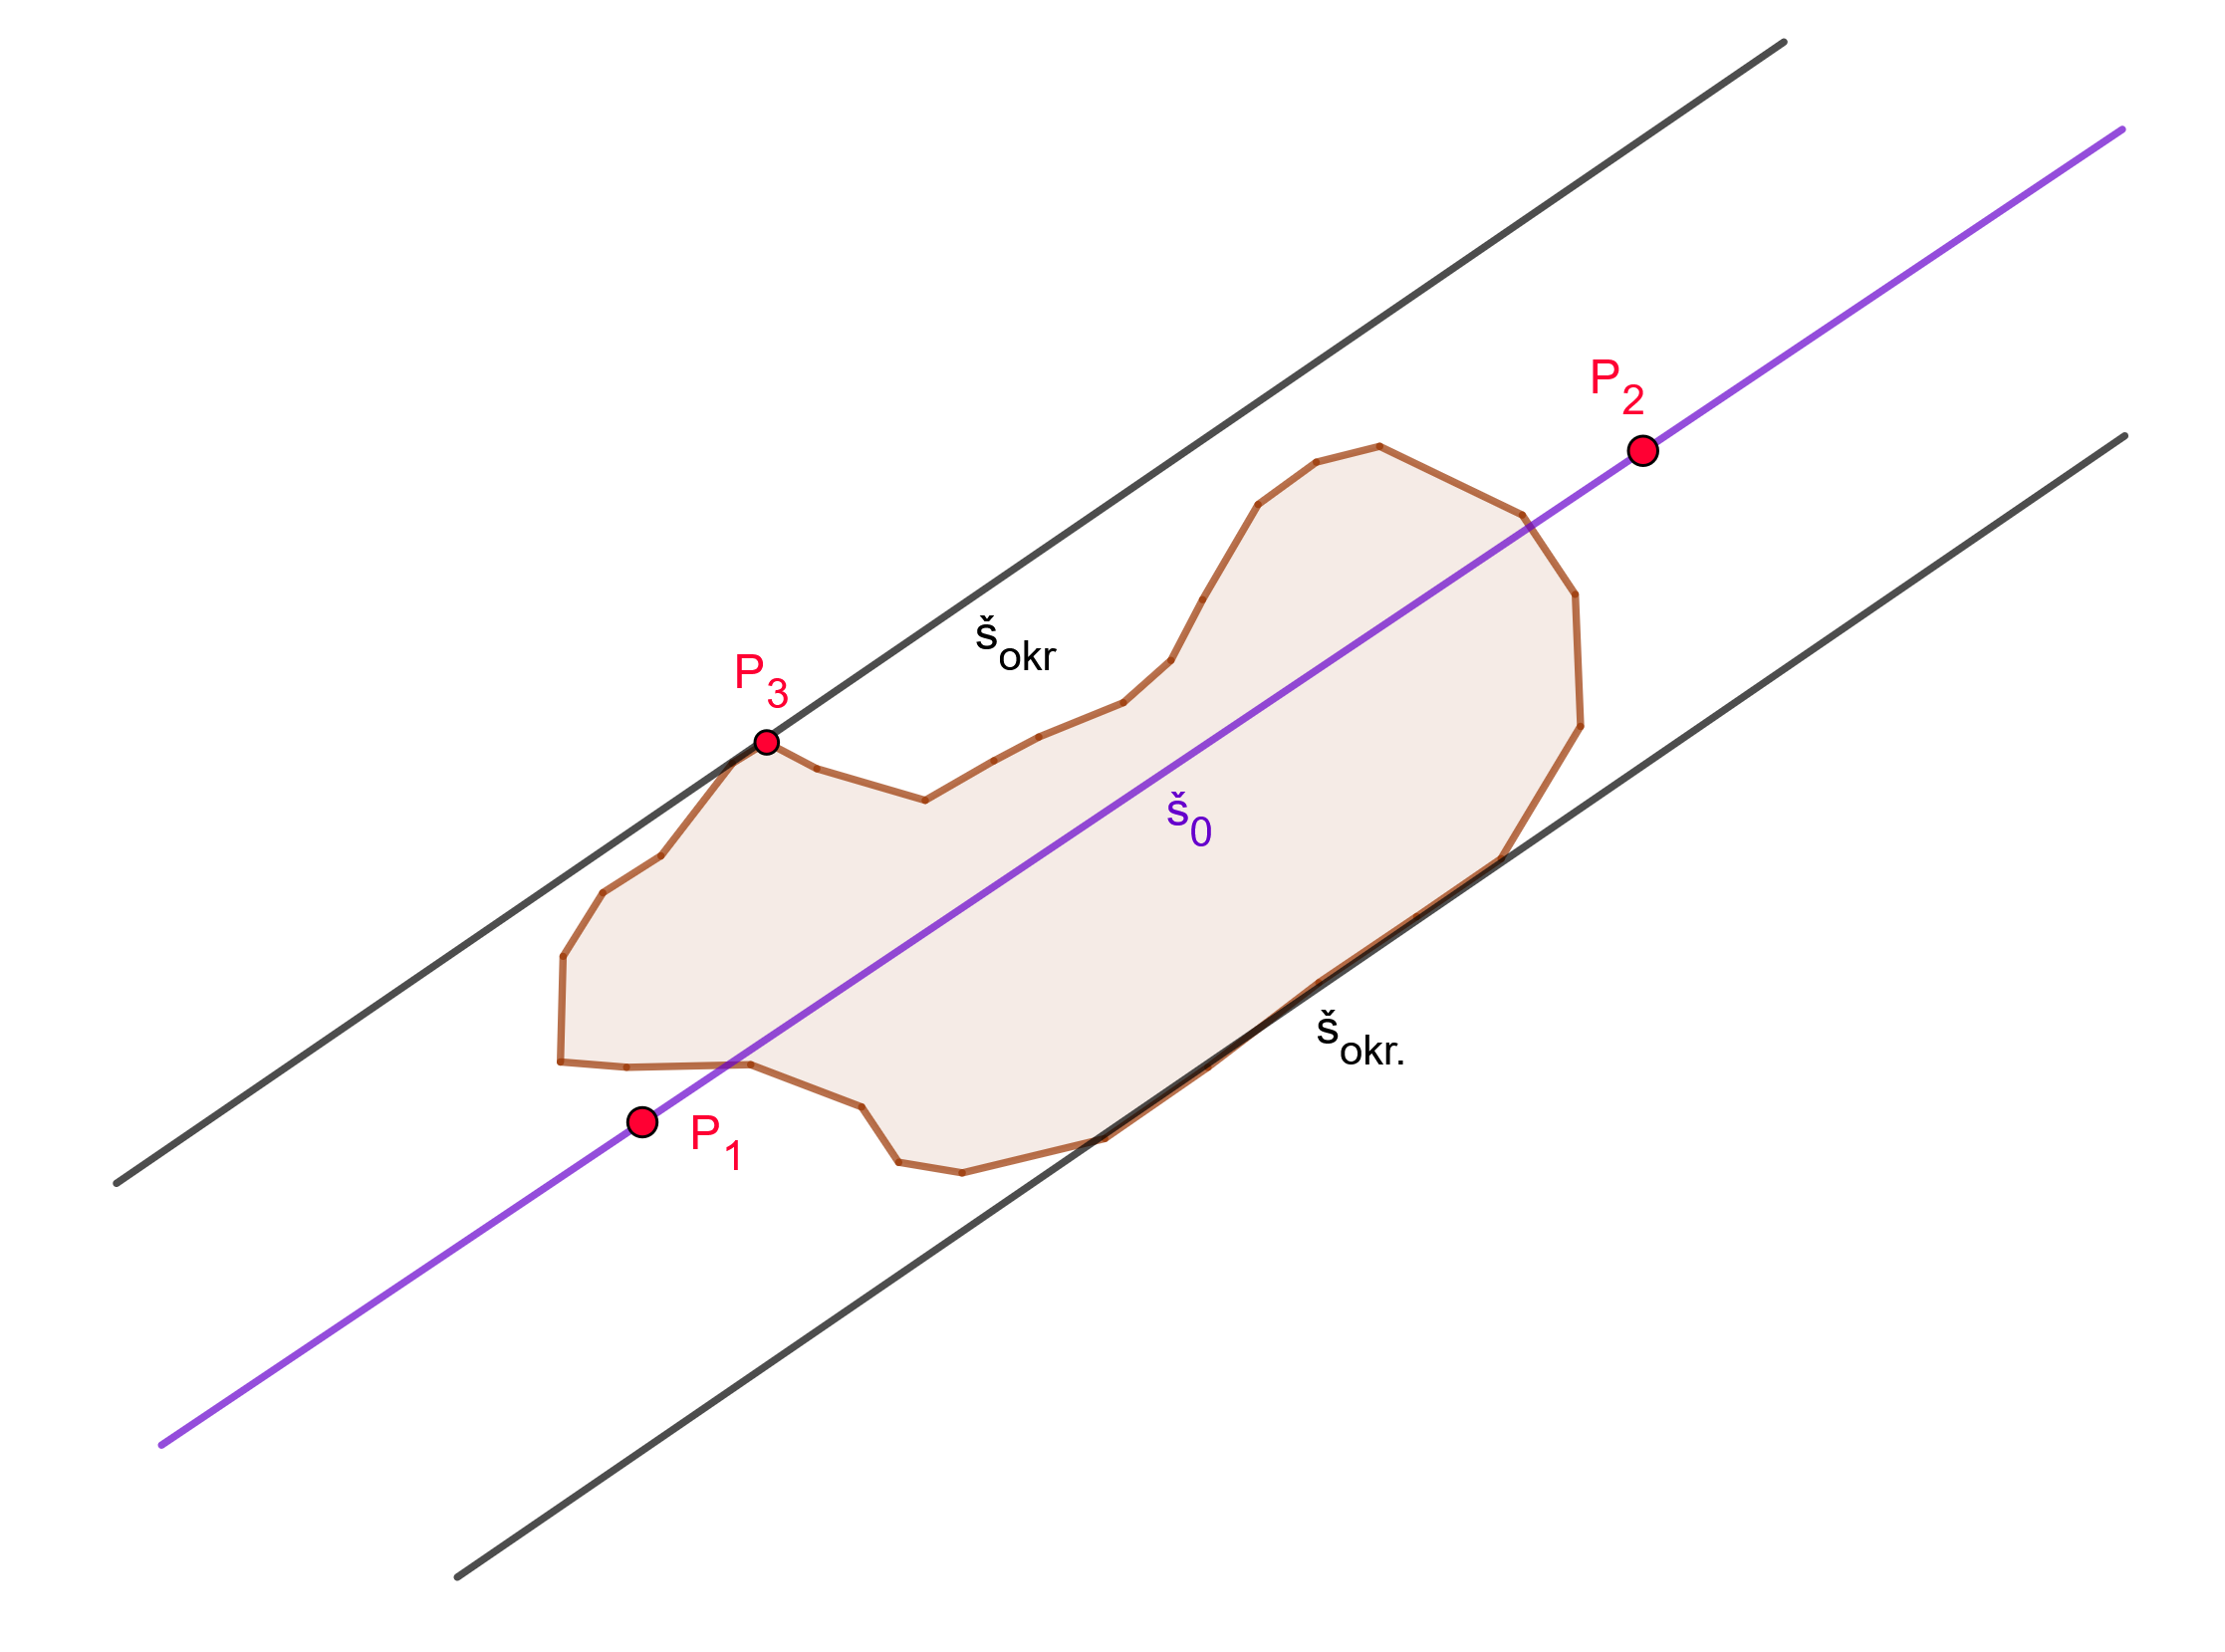
\includegraphics[scale=0.5]{figure/valec.png}
\captionsetup{justification=centering}
\caption{Znázornění volby válcového zobrazení v obecné poloze.}
\label{ob1}
\end{figure}

\subsection{Kuželové konformní zobrazení}
Lambertovo konformní kuželové zobrazení definujeme v obecné poloze rovnicemi:
$$\rho = \rho_0 \frac{\tan^c\left(\frac{\check{s}_0}{2} + 45^\circ\right)}{\tan^c\left(\frac{\check{s}}{2} + 45^\circ\right)}$$ 
$$\epsilon = c \cdot d$$ 
Pro nalezení konstant $\rho_0$ a $c$ uplatňujeme obdobnou logiku symetrie zkreslení. Požadujeme rovnost odchylek na okrajích a ve středu uvažovaného pásu ($m_r^s = m_r^j = 1 + \nu$ a $m_r^0 = 1 - \nu$). Součtem získáme podmínku $m_r^s + m_r^0 = 2$.

Úpravou zobrazovacích rovnic a dosazením okrajových hodnot odvodíme konstantu $\rho_0$:
$$\rho_0 = \frac{2R \cos \check{s}_0 \cos \check{s}_s \tan^c\left(\frac{\check{s}_s}{2} + 45^\circ\right)}{c\left[\cos \check{s}_0 \tan^c\left(\frac{\check{s}_0}{2} + 45^\circ\right) + \cos \check{s}_s \tan^c\left(\frac{\check{s}_s}{2} + 45^\circ\right)\right]}$$ 
Konstantu kužele $c$ definuje vztah zohledňující severní ($\check{s}_s$) a jižní ($\check{s}_j$) okrajovou rovnoběžku:
$$c = \frac{\log \cos \check{s}_s - \log \cos \check{s}_j}{\log \tan\left(\frac{\check{s}_j}{2} + 45^\circ\right) - \log \tan\left(\frac{\check{s}_s}{2} + 45^\circ\right)}$$ 
Přičemž platí $c = \sin \check{s}_0$. V praxi se území sevře do mezikruží tvořeného soustřednými kružnicemi o poloměrech $\rho_s$ a $\rho_j$. Zkreslení pak namátkově ověřujeme dosazením příslušných hodnot do vzorce $m = \frac{c\rho_s}{R \cos u_s}$.

 \begin{figure}[h!]
\centering
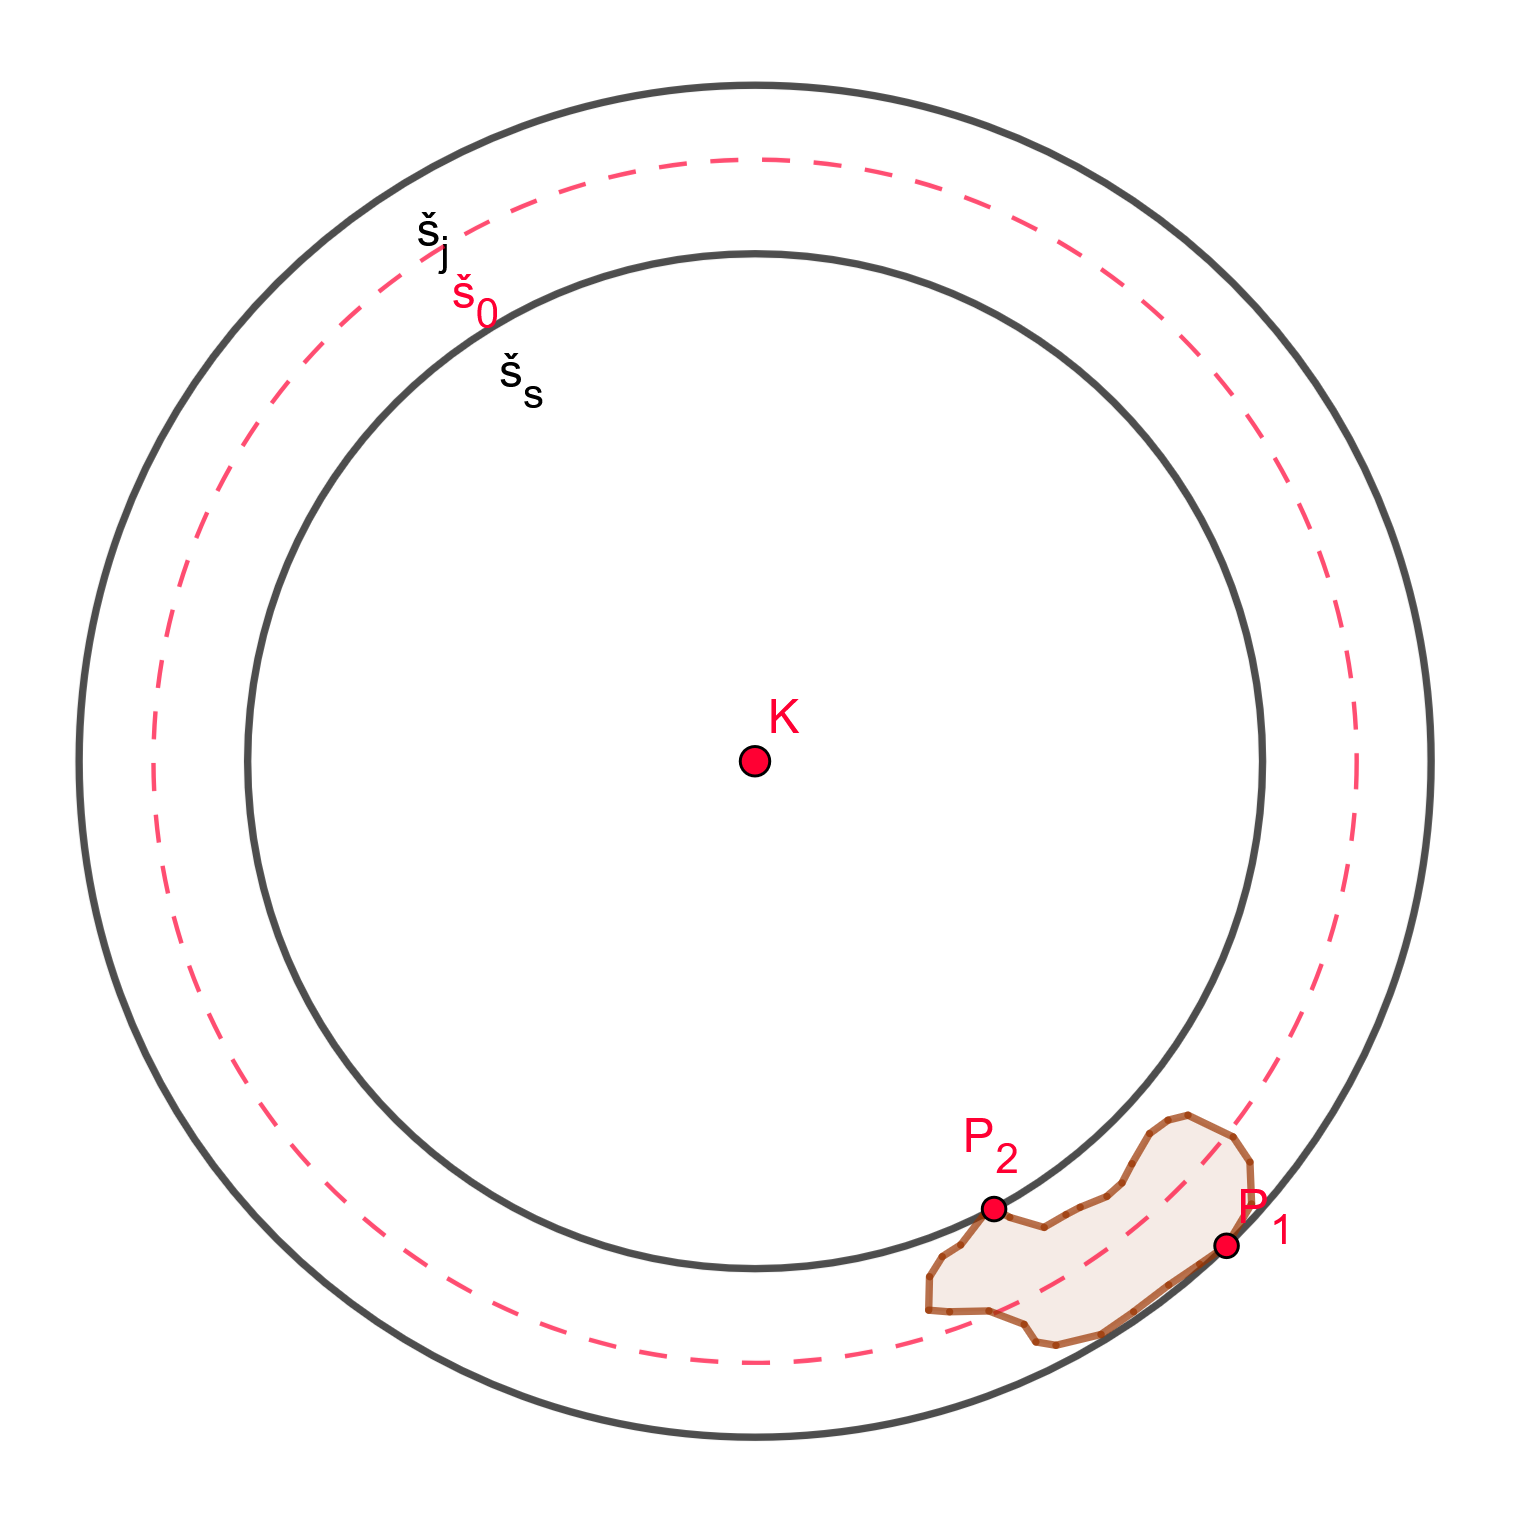
\includegraphics[scale=0.2]{figure/kuzel.png}
\captionsetup{justification=centering}
\caption{Znázornění volby kuželového zobrazení v obecné poloze.}
\label{ob2}
\end{figure}

\subsection{Azimutální konformní zobrazení}
Stereografickou projekci zapisujeme rovnicemi závislými na doplňku šířky do devadesáti stupňů ($\psi = 90^\circ - \check{s}$):
$$\rho = c \tan \frac{\psi}{2}, \quad \epsilon = d$$ 
Pokud je zobrazení definováno jednou nezkreslenou rovnoběžkou, konstanta $c$ odpovídá výrazu $2R \cos^2 \frac{\psi_0}{2}$. Délkové měřítko v libovolném bodě je pak dáno podílem:
$$m_r = \frac{\cos^2 \frac{\psi_0}{2}}{\cos^2 \frac{\psi}{2}}$$ 
Aby bylo zkreslení optimalizováno v celém pokrývaném rozsahu, zřekneme se nulového zkreslení přímo v pólu (kde zavedeme hodnotu $\mu = 1 - \nu$) a místo toho požadujeme, aby se odchylka v pólu a na jižní omezující kružnici lišila jen znaménkem.
Z rovnice $m_r^p + m_r^j = 2$  odvodíme optimální multiplikační konstantu $\mu$:
$$\mu = \frac{2 \cos^2 \frac{\psi_j}{2}}{1 + \cos^2 \frac{\psi_j}{2}}$$ 

 \begin{figure}[h!]
\centering
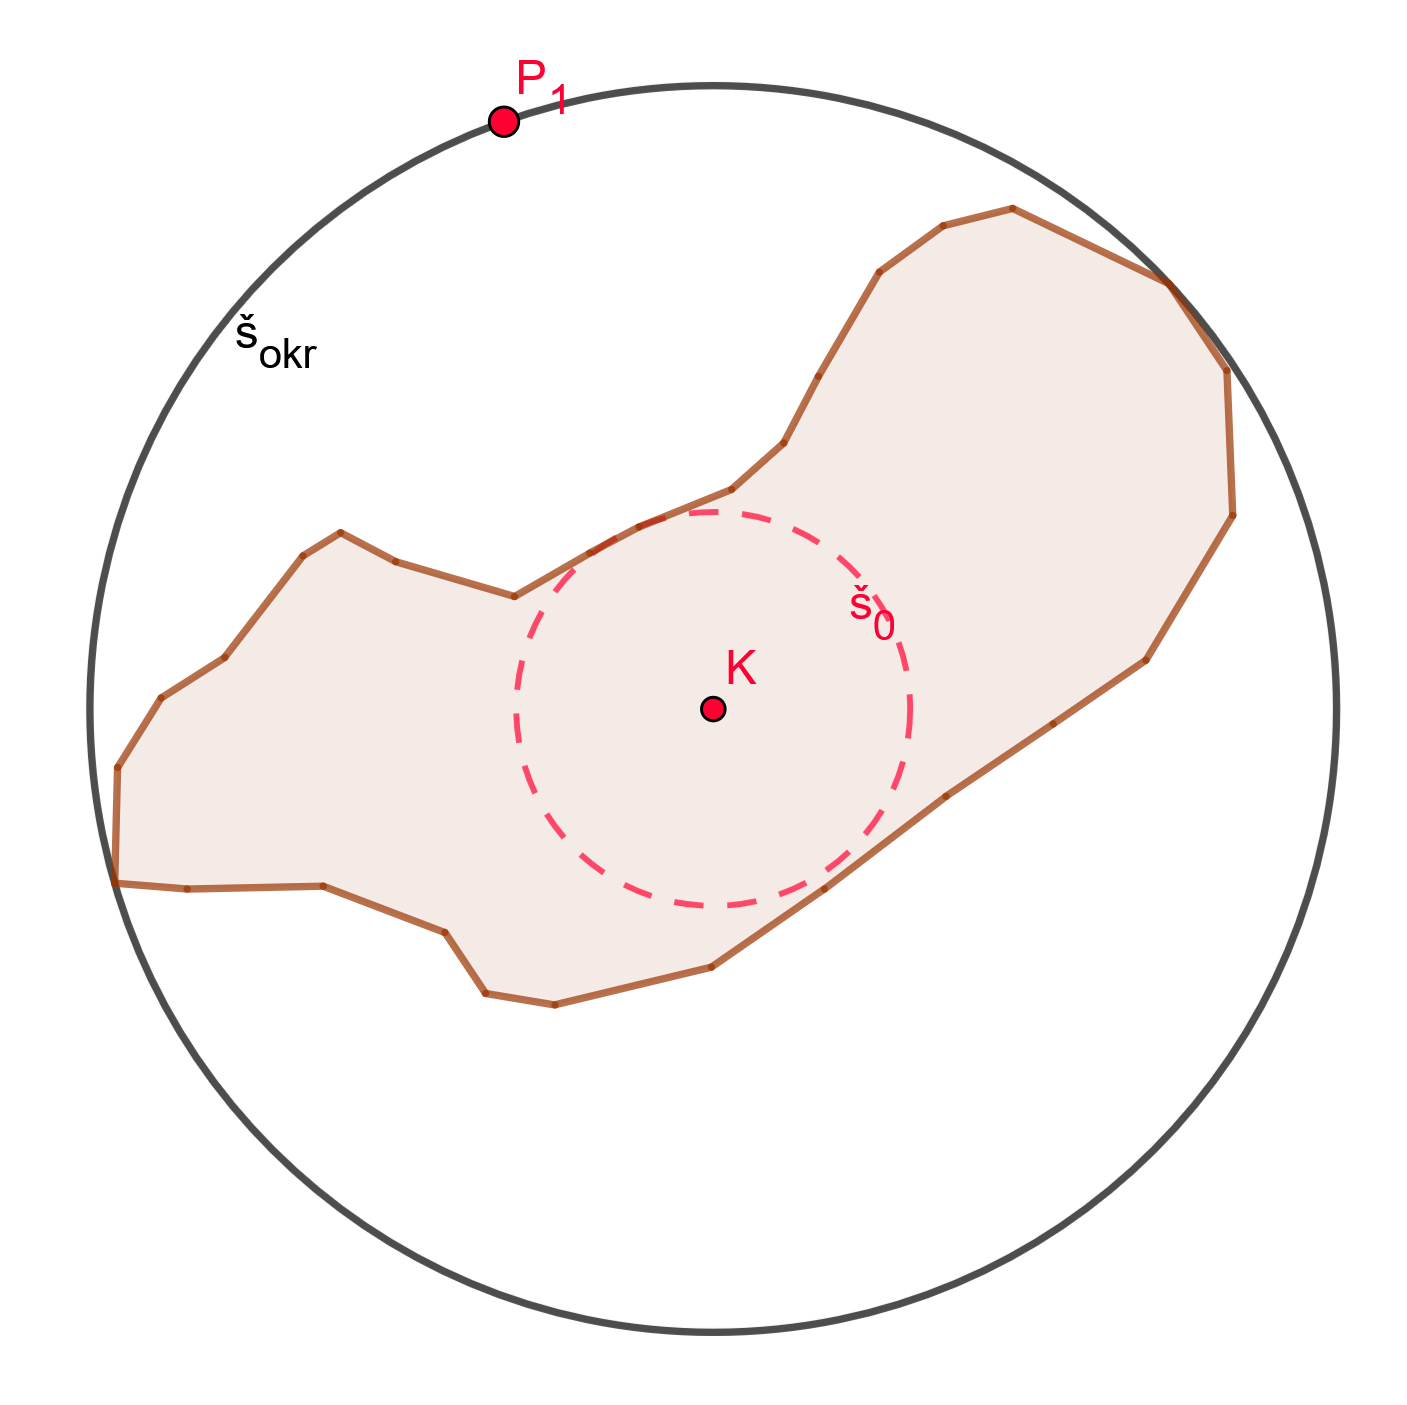
\includegraphics[scale=0.7]{figure/azimut.png}
\captionsetup{justification=centering}
\caption{Znázornění volby azimutálního zobrazení v obecné poloze.}
\label{ob3}
\end{figure}



\newpage
\section{Vypracování}
Pro zpracování úlohy byly zvoleny dva státy - jeden s dominantním směrem (Japonsko), druhý bez dominantního  směru (Německo). 
Pro oba tyto státy byly vytvořeny výše popsaná zobrazení a spočítany hodnoty zkreslení. 
Veškeré výpočty byly realizovány v programovacím jazyce Python s využitím knihoven \lstinline{shapefile}, \lstinline{math} a \lstinline{numpy}. 

Pro všechny výpočty bylo potřeba nahrát souřadnice bodů obou zemí uložených v shapefilech. 
To bylo provedeno s využitím knihovny \lstinline{shapefile}.
Níže je vyobrazen fragment kódu, který shapefile načítá a extrahuje jednotlivé body země. 
\begin{lstlisting}[language=Python, caption=Ukázka kódu pro načtení souřadnic bodů.]
    all_points = []
    
    #Extract all points from the shapefile
    with shapefile.Reader(shapefile_path) as shp:
        for shape_record in shp.shapeRecords():
            if not shape_record.shape.points:
                continue
            #shape.points are returned as (x, y) which is (longitude, latitude)
            all_points.extend(shape_record.shape.points)
\end{lstlisting}

\subsection{Válcové konformní zobrazení}
V rámci válcového konformního zobrazení byla exaktně spočtena dotyková rovnoběžka a pomocí analytické geometrie byl určen kartografický pól. 

\subsubsection*{Kartografický pól s využitím analytické geometrie}
Pro dosažení co nejnižšího maximálního zkreslení ve válcovém zobrazení musí být kartografický pól navržen tak, aby transformovaný kartografický rovník procházel nejdelší osou zadaného území. K nalezení této osy byl navržen algoritmus, který zkoumá vzdálenosti všech dvojic bodů tvořících tvar státu. 

Geografické souřadnice bodů byly nejprve převedeny do 3D kartézské soustavy na jednotkové referenční kouli ($R = 1$) pomocí vztahů:
$$ X = \cos u \cos v, \quad Y = \cos u \sin v, \quad Z = \sin u. $$
Následně algoritmus \lstinline{find_longest_axis} iteruje přes všechny body a hledá dvojici s maximální euklidovskou vzdáleností v trojrozměrném prostoru:
$$ d^2 = (X_2 - X_1)^2 + (Y_2 - Y_1)^2 + (Z_2 - Z_1)^2. $$
\begin{lstlisting}[language=Python, caption=Hledání nejdelší osy území.]
# Porovnani vsech bodu pro nalezeni nejdelsi spojnice
for i in range(len(cartesian_points)):
    x1, y1, z1 = cartesian_points[i]
    for j in range(i + 1, len(cartesian_points)):
        x2, y2, z2 = cartesian_points[j]
        
        # Vypocet 3D Euklidovske vzdalenosti
        dist_sq = (x2 - x1)**2 + (y2 - y1)**2 + (z2 - z1)**2
        
        if dist_sq > max_dist_sq:
            max_dist_sq = dist_sq
            p1 = unique_points[i]
            p2 = unique_points[j]
\end{lstlisting}
Jakmile jsou identifikovány body tvořící nejdelší osu ($P_1, P_2$), kartografický pól leží ve směru normálového vektoru $\vec{N}$ k rovině určené středem Země a těmito dvěma body. Tento vektor se získá pomocí vektorového součinu ($\times$) směrového vektoru osy ($\vec{P_2} - \vec{P_1}$) a polohového vektoru prvního bodu ($\vec{P_1}$):
$$ \vec{N} = (\vec{P_2} - \vec{P_1}) \times \vec{P_1}. $$
Knihovna \lstinline{numpy} umožňuje tento výpočet provést velmi jednodušše:
\begin{lstlisting}[language=Python, caption=Vektorový součin a normalizace pro nalezení pólu.]
# Vypocet vektoroveho soucinu
N_G = cross([XN2-XN1, YN2-YN1, ZN2-ZN1], [XN1, YN1, ZN1])

# Normalizace vektoru
n_G = N_G / linalg.norm(N_G)
\end{lstlisting}

Po zisku normalizovaného vektoru $\vec{n} = (n_x, n_y, n_z)$ je finálním krokem zpětná konverze do sférických úhlů (geografických souřadnic pólu $u_k, v_k$), čímž získáme přesnou polohu pólu bez nutnosti grafického odhadování v GIS softwaru:
$$ u_k = \arcsin(n_z), \quad v_k = \text{atan2}(n_y, n_x). $$

\subsubsection*{Exaktní výpočet dotykové rovnoběžky}
Pro výpočet optimální dotykové (nezkreslené) rovnoběžky $\check{s}_0$ je nezbytné nalézt bod s maximální absolutní hodnotou kartografické šířky (tedy bod na okraji území). Pro všechny hraniční body státu byla vypočtena jejich kartografická šířka $\check{s}$ pomocí sférické trigonometrie:
$$ \sin \check{s} = \sin u \sin u_k + \cos u \cos u_k \cos(v - v_k). $$

V programovacím jazyce Python byl tento matematický vztah implementován tímto způsobem:

\begin{lstlisting}[language=Python, caption=Výpočet kartografické šířky.]
# Prevod stupnu na radiany
u = radians(lat)
v = radians(lon)

# Vypocet kartograficke sirky (s)
s = asin(sin(u)*sin(uk) + cos(u)*cos(uk)*cos(v-vk))
\end{lstlisting}

Pro iterativní prohledání všech bodů území byla využita vlastní funkce \lstinline{Find_Boundary_Points} Vstupem do této funkce jsou geografické souřadnice kartografického pólu ($u_k, v_k$), vůči kterému se určuje nová kartografická šířka $\check{s}$ pro každý bod státu (s geografickými souřadnicemi $u, v$) na základě sférické kosinové věty:
$$ \sin \check{s} = \sin u \sin u_k + \cos u \cos u_k \cos(v - v_k). $$


Během iterace přes všechny unikátní body území algoritmus uchovává extrémní hodnoty v kladném i záporném směru od nového kartografického rovníku (\lstinline{s_max_positive} a \lstinline{s_max_negative}). 
Bod s absolutně největší odchylkou $\check{s}_{okr} = \max(|\check{s}_i|)$ je následně použit k definování polohy standardní rovnoběžky $\check{s}_0$. Tento krok zaručuje, že zkreslení bude na obou okrajích mapy symetrické. Výpočet se řídí vztahem:
$$ \cos \check{s}_0 = \frac{2 \cos \check{s}_{okr}}{1 + \cos \check{s}_{okr}} $$

V kódu je tento vztah reprezentován samostatnou funkcí:
\begin{lstlisting}[language=Python, caption=Výpočet dotykové rovnoběžky.]
def calculate_standard_parallel(s_max_rad):
    numerator = 2 * cos(s_max_rad)
    denominator = 1 + cos(s_max_rad)
    cos_s0 = numerator / denominator
    return acos(cos_s0)
\end{lstlisting}

\subsubsection*{Výsledky}
V tabulkách~\ref{table:1} až~\ref{table:3}  jsou vypsány souřadnice kartografického pólu a jednotlivých bodů:
    \begin{table}[h!]
        \centering
        \begin{tabular}{|p{3cm}|p{3cm}|p{3cm}|} 
         \hline
            Bod & \textit{u}  & \textit{v} \\
            \hline
            Pól  &   13.148365  & 117.826155 \\
            \hline
            $P_1$   &  47.520502 &  13.046055\\
            \hline
            $P_2$   &  54.977031 & 8.355316 \\
            \hline
            $P_3$   &  53.928652 & 14.226302 \\
            \hline
            $P_4$   &  47.589878 & 7.589039 \\
            \hline
        \end{tabular}
        \caption{Souřadnice bodů a pólu [$^\circ$] pro Německo.}
\label{table:1}
    \end{table}
 

    \begin{table}[h!]
        \centering
        \begin{tabular}{|p{3cm}|p{3cm}|p{3cm}|} 
         \hline
            Bod & \textit{u}  & \textit{v} \\
            \hline
            Pól  &   -54.281256  & 105.791691 \\
            \hline
            $P_1$   &  33.339523 &  129.602363 \\
            \hline
            $P_2$   &  19.269814 & 166.701270\\
            \hline
            $P_3$   &  31.063241 & 130.742429 \\
            \hline
            $P_4$   &  45.459198 & 141.866284 \\
            \hline
        \end{tabular}
        \caption{Souřadnice bodů a pólu [$^\circ$] pro Japonsko (bez jižních ostrovů).}
\label{table:2}
    \end{table}

    \begin{table}[h!]
        \centering
        \begin{tabular}{|p{3cm}|p{3cm}|p{3cm}|} 
         \hline
            Bod & \textit{u}  & \textit{v} \\
            \hline
            Pól  &   65.493639  & -53.221546 \\
            \hline
            $P_1$   &  19.269814 &  166.701270 \\
            \hline
            $P_2$   &  24.457313 & 122.919561 \\
            \hline
            $P_3$   &  45.459198 & 141.866284 \\
            \hline
            $P_4$   &  20.380988 & 136.040071 \\
            \hline
        \end{tabular}
        \caption{Souřadnice bodů a pólu [$^\circ$] pro Japonsko.}
\label{table:3}
    \end{table}

\newpage
\textbf{Zhodnocení zkreslení} \\
Vypočtené hodnoty délkového zkreslení $\nu$ poukazují na geometrické limity tohoto zobrazení. Zatímco u kompaktního území Německa se maximální hodnoty zkreslení na severním okraji ($0,325$), jižním okraji ($0,878$) a kartografickém rovníku ($-0,878$) drží v přijatelných symetrických mezích, u Japonska se projevuje výrazná asymetrie. 

Pro pevninské Japonsko dosahuje zkreslení na jižním okraji hodnoty $31,859$ oproti $0,297$ na okraji severním. Při zahrnutí jižních ostrovů se tato asymetrie překlápí a extrémně narůstá – severní okraj vykazuje zkreslení $74,095$, zatímco jižní pouze $1,120$. 

    
\subsection{Kuželové konformní zobrazení}
V rámci kuželového konformního zobrazení byl pomocí analytické geometrie určen kartografický pól. 




\subsubsection*{Kartografický pól s využitím analytické geometrie}

Pro kuželové zobrazení je kartografický pól matematicky definován jako normálový vektor k rovině řezu (malé kružnici), která je rovnoběžná s převažující orientací zájmového území. K jednoznačnému definování libovolné roviny ve 3D prostoru, která neprochází středem souřadnicové soustavy, jsou zapotřebí právě tři body ležící na povrchu referenční koule.

Aby rovina co nejpřesněji reprezentovala celkový sklon a orientaci státu, nesmí jít o náhodné body z vnitrozemí. Množina všech bodů území byla proto nejprve algoritmicky zredukována pouze na vnější hraniční body pomocí nalezení konvexní obálky (Convex Hull). K tomu byl  implementován Jarvis Scan (Gift Wrapping algorithm), který postupně „obaluje“ množinu bodů na základě výpočtu úhlů mezi vektory.

\begin{lstlisting}[language=Python, caption=Redukce bodů pomocí konvexní obálky.]
def createCH(points):
    pol = list(set(points))
    ch = []
    # Nalezeni nejnizsiho bodu (pocatecni bod obalky)
    q = min(pol, key=lambda k: k[1])
    # ... (iterativni hledani bodu s maximalnim uhlem) ...
    return ch

# Aplikace na nactena data
boundary_points = createCH(all_points)
\end{lstlisting}

Z takto získané uspořádané množiny hraničních bodů byly vybrány tři prostorově distribuované body ($P_1, P_2, P_3$). Aby rovina protínala území stabilně a nedošlo k výběru bodů ležících příliš blízko u sebe, byly body vybrány s rovnoměrným odstupem odpovídajícím třetinám délky pole hraničních bodů. Tyto body byly následně transformovány z geografických do 3D kartézských souřadnic ($X, Y, Z$).

V rovině řezu byly z těchto tří bodů vytvořeny dva směrové vektory sdílející společný počátek v bodě $P_1$:
$$ \vec{V_1} = P_2 - P_1, \quad \vec{V_2} = P_3 - P_1. $$

Směr kartografického pólu pak jednoznačně určuje normálový vektor $\vec{N}$ k této rovině, který byl vypočten pomocí vektorového součinu obou směrových vektorů v knihovně \lstinline{numpy}:
$$ \vec{N} = \vec{V_1} \times \vec{V_2}. $$

\begin{lstlisting}[language=Python, caption=Tvorba roviny a výpočet normálového vektoru.]
# Vytvoreni smerovych vektoru lezicich v rovine rezu
V1 = [X2 - X1, Y2 - Y1, Z2 - Z1]
V2 = [X3 - X1, Y3 - Y1, Z3 - Z1]

# Vektorovy soucin pro nalezeni kolmice (polu)
N = np.cross(V1, V2)
\end{lstlisting}

Při výpočtu vektorového součinu v prostoru je však nutné ošetřit směr normálového vektoru. Výsledný normálový vektor může směřovat buď ven z referenční koule (správný pól), nebo dovnitř skrz střed Země na opačnou polokouli, v závislosti na tom, zda byly body $P_1, P_2, P_3$ vybrány po směru nebo proti směru hodinových ručiček. 

Tento geometrický problém byl v kódu vyřešen  pomocí skalárního součinu. Skalární součin vypočtené normály $\vec{N}$ a polohového vektoru středu území (např. $\vec{P_1}$) odhalí vzájemnou orientaci. Je-li výsledek záporný, úhel mezi vektory je větší než $90^\circ$, což znamená, že pól směřuje na odvrácenou stranu planety. V takovém případě byl vektor jednoduše invertován ($\vec{N} = -\vec{N}$).

\begin{lstlisting}[language=Python, caption=Korekce směru pólu pomocí skalárního součinu.]
# Kontrola orientace pomoci skalarniho soucinu
# Pokud pol ukazuje opacnym smerem skrz Zemi, invertujeme jej
if np.dot(N, [X1, Y1, Z1]) < 0:
    N = -N
\end{lstlisting}

Posledním krokem po úspěšné orientaci vektoru byla jeho normalizace na jednotkovou délku ($\vec{n} = \vec{N} / |\vec{N}|$) a zpětný převod ze 3D kartézské soustavy do geografických souřadnic $u_k, v_k$ pomocí  funkcí $\arcsin$ a $\text{atan2}$. Tím byla analyticky a zcela exaktně získána poloha optimálního kartografického pólu pro kuželové zobrazení.

\subsubsection*{Výsledky}
V tabulkách~\ref{table:4} až~\ref{table:6}  jsou vypsány souřadnice kartografického pólu a jednotlivých bodů:

    \begin{table}[h!]
        \centering
        \begin{tabular}{|p{3cm}|p{3cm}|p{3cm}|} 
         \hline
            Bod & \textit{u}  & \textit{v} \\
            \hline
            Pól  &   50.741239 & 11.541305 \\
            \hline
            $P_1$   &  50.318028 &  12.100900\\
            \hline
            $P_2$   &  54.97703 & 8.355316 \\
            \hline
        \end{tabular}
        \caption{Souřadnice bodů a pólu [$^\circ$] pro Německo.}
\label{table:4}
    \end{table}


    \begin{table}[h!]
        \centering
        \begin{tabular}{|p{3cm}|p{3cm}|p{3cm}|} 
         \hline
            Bod & \textit{u}  & \textit{v} \\
            \hline
            Pól  &    28.747167  & 149.983177 \\
            \hline
            $P_1$   &  35.198779 &  140.375467 \\
            \hline
            $P_2$   &  33.230916 & 129.576257\\
            \hline
         
        \end{tabular}
        \caption{Souřadnice bodů a pólu [$^\circ$] pro Japonsko (bez jižních ostrovů).}
\label{table:5}
    \end{table}



    \begin{table}[h!]
        \centering
        \begin{tabular}{|p{3cm}|p{3cm}|p{3cm}|} 
         \hline
            Bod & \textit{u}  & \textit{v} \\
            \hline
            Pól  &   25.213941  &  145.466147 \\
            \hline
            $P_1$   &  27.027972 &  142.239838 \\
            \hline
            $P_2$   &  45.447871 & 141.002785 \\
            \hline
    
        \end{tabular}
        \caption{Souřadnice bodů a pólu [$^\circ$] pro Japonsko.}
\label{table:6}
    \end{table}
\newpage
\textbf{Zhodnocení zkreslení} \\
Získané hodnoty zkreslení $\nu$  plně reflektují úspěšné splnění zadané podmínky symetrie, kdy se zkreslení na obou okrajových rovnoběžkách i ve středové rovnoběžce pásu liší pouze znaménkem ($m_r^s = m_r^j = 1 + \nu, m_r^0 = 1 - \nu$). Toto zobrazení vykazuje nejnižší celkové zkreslení ze všech tří testovaných variant. 

Pro Německo je maximální zkreslení $\nu_{max}$ symetricky rozloženo na hodnotách  $\pm 0,354087$. Pro pevninské Japonsko činí odchylka pouhých $\pm 1,121$ a ani po přidání všech vzdálených jižních ostrovů nepřesahuje $\pm 6,046$. To ukazuje, že vhodně orientovaný kužel protínající referenční plochu dokáže ideálně optimalizovat i velice protáhlé a asymetrické tvary států.

\subsection{Azimutální konformní zobrazení}
V rámci azimutálního konformního zobrazení byl kartografický pól určen jako střed opsané kružnice s minimálním poloměrem. 


\subsubsection*{Kartografický pól jako střed opsané kružnice}
Optimalizace azimutálního zobrazení (v tomto případě stereografické projekce) spočívá v minimalizaci maximálního délkového zkreslení na okraji zájmového území. Z geometrického hlediska tato úloha odpovídá nalezení \textbf{nejmenší opsané kružnice} (Minimum Enclosing Circle – MEC), která v sobě uzavře všechny body definující daný stát. Střed této kružnice $K = [u_k, v_k]$ se stává optimálním kartografickým pólem a její poloměr $R$ určuje hranici maximálního zkreslení.

Vzhledem k vysokému počtu bodů v souborech shapefile by byl výpočet MEC nad všemi body výpočetně neefektivní. Proto i zde bylo využito algoritmu pro určení konvexní obálky.


Nad takto získanými hraničními body (\lstinline{boundary_points}) byl následně realizován algoritmus pro nalezení MEC. Matematicky je nejmenší opsaná kružnice jednoznačně definována buď dvěma body (tvořícími její průměr), nebo třemi body (tvořícími vrcholy opsaného trojúhelníku). Algoritmus proto iteruje přes všechny možné dvojice a trojice hraničních bodů.

Pro každou kandidátní kružnici je nutné ověřit její validitu – tedy zda jsou všechny ostatní body území obsaženy uvnitř této kružnice. V kódu byla tato kontrola realizována funkcí \lstinline{is_valid_circle}:

\begin{lstlisting}[language=Python, caption=Kontrola validity kandidátní kružnice.]
def is_valid_circle(center, radius, points):
    for p in points:
        # Vypocet euklidovske vzdalenosti bodu od stredu
        if hypot(p[0] - center[0], p[1] - center[1]) > radius + 1e-5:
            return False
    return True
\end{lstlisting}

Pokud je kružnice definována dvěma body $P_i, P_j$, její střed leží v jejich geometrickém středu a poloměr je roven polovině jejich vzdálenosti. V případě tří bodů $A, B, C$ se jedná o nalezení středu kružnice opsané trojúhelníku. Ten byl vypočten pomocí soustavy lineárních rovnic odvozených z determinantů:

\begin{lstlisting}[language=Python, caption=Výpočet středu kružnice ze tří bodů.]
def circle_from_3_points(p1, p2, p3):
    temp = p2[0]*p2[0] + p2[1]*p2[1]
    bc = (p1[0]*p1[0] + p1[1]*p1[1] - temp) / 2
    cd = (temp - p3[0]*p3[0] - p3[1]*p3[1]) / 2
    det = (p1[0] - p2[0]) * (p2[1] - p3[1]) - (p2[0] - p3[0]) * (p1[1] - p2[1])
    
    cx = (bc*(p2[1] - p3[1]) - cd*(p1[1] - p2[1])) / det
    cy = ((p1[0] - p2[0])*cd - (p2[0] - p3[0])*bc) / det
    radius = hypot(p2[0] - cx, p2[1] - cy)
    return (cx, cy), radius
\end{lstlisting}

Výsledný kartografický pól $[u_k, v_k]$ je středem té kružnice, která prošla testem validity a zároveň vykazovala absolutně nejmenší poloměr ze všech testovaných kombinací. Tento analytický přístup zaručuje, že stereografická projekce bude mít pro daný stát (např. Německo či Japonsko) nejmenší možný rozptyl délkového zkreslení.

\begin{figure}[h!]
\centering
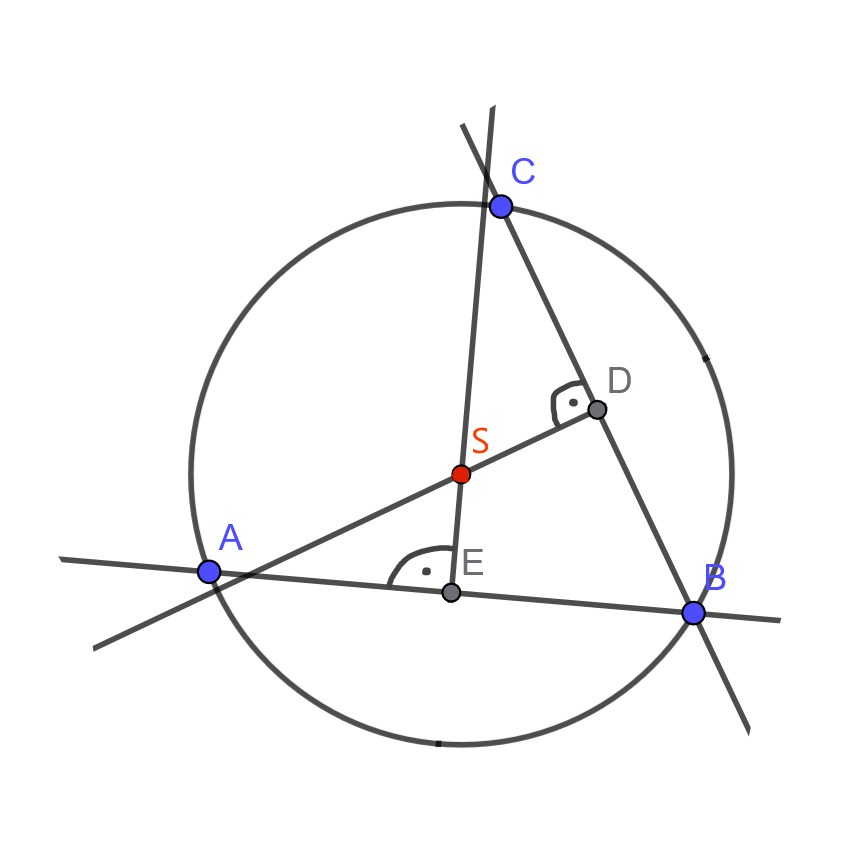
\includegraphics[scale=0.5]{figure/3pointcircle.png}
\captionsetup{justification=centering}
\caption{Geometrický princip kružnice opsané třem hraničním bodům území.}
\label{ob4}
\end{figure}




\subsubsection*{Výsledky}
V tabulkách~\ref{table:7} až~\ref{table:9}  jsou vypsány souřadnice kartografického pólu a bodu:

    \begin{table}[h!]
        \centering
        \begin{tabular}{|p{3cm}|p{3cm}|p{3cm}|} 
         \hline
            Bod & \textit{u}  & \textit{v} \\
            \hline
            Pól  &   51.185011 & 10.501071 \\
            \hline
            $P_1$   &  47.561113 &  7.634097\\
            \hline

        \end{tabular}
        \caption{Souřadnice bodu a pólu [$^\circ$] pro Německo.}
\label{table:7}
    \end{table}


    \begin{table}[h!]
        \centering
        \begin{tabular}{|p{3cm}|p{3cm}|p{3cm}|} 
         \hline
            Bod & \textit{u}  & \textit{v} \\
            \hline
            Pól  &   26.688015  & 148.297200 \\
            \hline
            $P_1$   &  45.459198 &  141.866284 \\
            \hline

         
        \end{tabular}
        \caption{Souřadnice bodu a pólu [$^\circ$] pro Japonsko (bez jižních ostrovů).}
\label{table:8}
    \end{table}



    \begin{table}[h!]
        \centering
        \begin{tabular}{|p{3cm}|p{3cm}|p{3cm}|} 
         \hline
            Bod & \textit{u}  & \textit{v} \\
            \hline
            Pól  &   23.696010  & 145.027534 \\
            \hline
            $P_1$   &  45.447871 &  141.002785 \\
            \hline

    
        \end{tabular}
        \caption{Souřadnice bodu a pólu [$^\circ$] pro Japonsko.}
\label{table:9}
    \end{table}

\textbf{Zhodnocení zkreslení} \\
Vypočtené hodnoty $\nu$  ukazují, že i v rámci azimutálního zobrazení se podařilo exaktně dodržet optimalizační požadavek – odchylka v pólu a na omezující kružnici opsané se liší výhradně znaménkem. Území s nulovým zkreslením v tomto případě tvoří standardní kružnici ležící mezi pólem a hranicí zobrazení.

U sféricky kompaktního Německa je maximální zkreslení na okraji nepatrné ($\nu_1 = 0,632$) a zcela vyvažuje kompresi ve středu mapy ($\nu_2 = -0,632$). U Japonska, vlivem značné polohové vzdálenosti nejzazších bodů od vypočteného středu opsané kružnice, zkreslení logicky a výrazně narůstá. Pro pevninskou část dosahuje symetrických $\pm 14,490$ a po zahrnutí odlehlých ostrovů stoupá poloměr opsané kružnice natolik, že zkreslení dosáhne $\pm 18,533$.



\newpage
\section{Závěr}
Tato práce zkoumala vhodnost a analyzovala délkové zkreslení konformních zobrazení v obecné poloze (válcového, kuželového a azimutálního). Cílem bylo optimalizovat parametry pro stát bez dominantního směru (Německo) a stát s dominantním směrem (Japonsko), s důrazem na symetrii maximálních odchylek na okrajích a ve středu plochy.

Na základě diskutovaných hodnot z jednotlivých podkapitol lze zobecnit následující závěry k využitelnosti zobrazení:

\begin{itemize}
    \item \textbf{Pro území bez dominantního směru (Německo):} 
    Díky kompaktnímu, téměř kruhovému tvaru tohoto státu jsou aplikovatelná všechna tři zobrazení. Ve všech případech se maximální deformace drží pod  hodnotou $1 \cdot 10^{-3}$. Pokud bychom však měli zvolit nejlepší zobrazení, je jím \textbf{konformní kuželové zobrazení v obecné poloze}, které poskytlo nejmenší celkové zkreslení ($\pm 0,354 \cdot 10^{-3}$).
    
    \item \textbf{Pro území s dominantním směrem (Japonsko):} 
    Pro tento asymetrický, podélně orientovaný tvar rozprostírající se přes velkou oblast je jednoznačně nejvhodnější volbou \textbf{konformní kuželové zobrazení v obecné poloze}. To jako jediné spolehlivě pojalo i okrajové jižní ostrovy, perfektně dodrželo zadáním vyžadovanou symetrii extrémů zkreslení ($m_r^s = m_r^j = 1 + \nu, m_r^0 = 1 - \nu$) a udrželo celkové deformace na  $\pm 6,046 \cdot 10^{-3}$. Válcové zobrazení u asymetrických částí naprosto selhalo v udržení symetrických odchylek na okrajích a azimutální zobrazení generovalo zbytečně obrovskou opsanou kružnici, čímž neefektivně maximalizovalo chybu na $\pm 18,533 \cdot 10^{-3}$.
\end{itemize}
